\documentclass{livre}

\titre{Patchwork combinatoire de courbes algébriques}
\auteur{Raphaël \textsc{Alexandre}, Thomas \textsc{Mordant} \\ Encadré par : Ilia \textsc{Itenberg}}

\begin{document}

\tableofcontents

\newpage
\chapter{Introduction du problème}

Avant le propos central de ce texte, nous allons essayer d'exposer le problème étudié ainsi que de poser les premières notations utilisées.

\section{Le seizième problème de \textsc{Hilbert}}

Le problème est le suivant. \'Etant donné une polynôme homogène $F(x_0,x_1,x_2)$ à coefficients réels et de degré $d$, quelles sont les qualités topologiques de ses zéros dans le plan projectif réel, $\P^{2}(\R)$ ? 

Par la suite, nous supposerons toujours que les zéros de $F$ sont non-singuliers.

Nous désignerons par $\R F$ l'ensemble des zéros de $F$, qui a alors  naturellement une structure de variété lisse. Une variété lisse fermée de dimension $1$ dans un espace compact est une union de cercles. Ainsi, $\R F$ sera une collection de cercles.


\paragraph{En dimension $1$}En prenant $d=1$, nous observons que \[ F(x_0,x_1,x_2) = ax_0 + bx_1+cx_2 \]avec $a,b,c\in \R$. Ainsi, $\R F$ est une droite de $\R^{2}$. Son plongement dans $\P^{2}(\R)$ est un grand cercle.

\subsection*{Plongements de $\R^{2}$ dans $\P^{2}(\R)$}

Il est utile de garder à l'esprit que deux plongements possibles dans $\P^{2}(\R)$ donnent lieu à un cercle :

\begin{itemize}
\item le plongement d'une droite de $\R^{2}$ (qui donne un grand cercle qui intersecte la droite à l'infini en un point) ;
\item le plongement d'une conique de $\R^{2}$ (que nous appellerons \textit{ovale}).\note{Quelques doutes dessus, il faudrait vérifier si c'est le plongement d'une conique ou d'autre chose ...}
\end{itemize}

Le plongement d'un ovale divise $\P^{2}(\R)$ en deux régions non connectées : une boule et un ruban de \textsc{Möbius}.\note{Est-ce que c'est aussi vrai pour les grands cercles ?}

\paragraph{En dimension $2$}Si on revient au problème initial, pour $d=2$ nous avons $F$ qui décrit une conique de $\P^{2}(\R)$, c'est donc ou bien un ovale ou bien l'ensemble vide (ce qui se produit lorsque $F$ est définie).

\lemme{ 
Nous montrerons que :
\begin{itemize}
\item lorsque $d$ est pair, $\R F$ est une réunion d'ovales ;
\item lorsque $d$ est impair, $\R F$ est la réunion d'une droite et d'ovales.
\end{itemize}
}{}

\paragraph{En dimension $4$}La classification pour $d=4$ nous donne la distinction de cas suivante sur la composition de $\R F$:
\begin{itemize}
\item cela peut être l'ensemble vide ;
\item un, ou deux, ou trois, ou quatre ovales ;
\item un ovale dans un autre tel que dans la figure qui suit.
\end{itemize}

\begin{figure}[H]
\begin{center}
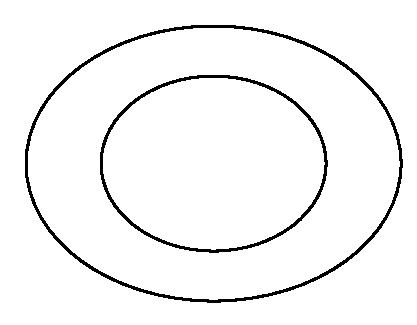
\includegraphics[scale=0.6]{fig1}
\end{center}
\caption{Lorsque $d=4$, un ovale peut être dans un autre}\label{fig1}
\end{figure}

Mais le cas suivant est impossible :
\begin{figure}[H]
\begin{center}
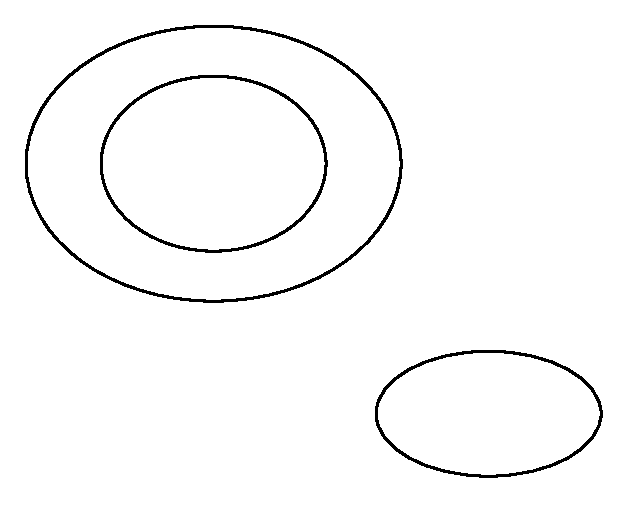
\includegraphics[scale=0.6]{fig2}
\end{center}
\caption{Ceci est impossible}
\end{figure}
En effet, si on trace une droite qui coupe chacun des ovales en deux points, on obtient $6$ points d'intersections alors que le degré de l'équation sous-jacente est de $4$.
\begin{figure}[H]
\begin{center}
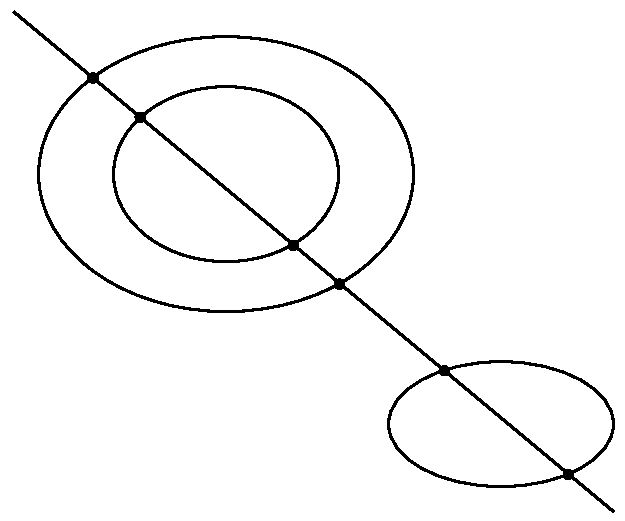
\includegraphics[scale=0.55]{fig3}
\end{center}
\caption{Les six points d'intersections contredisent $d=4$}
\end{figure}

On procède de même avec le cas où nous aurions $5$ ovales. Par leurs $5$ centres passe une conique et l'intersection est de $10$ points alors qu'il devrait y en avoir au plus $4\times 2 = 8$.

\end{document}
